\documentclass[journal, draftcls]{IEEEtran}

\usepackage{graphicx}
\usepackage{titling}
\usepackage{setspace}
\usepackage{geometry}
\usepackage{tikz}
\usepackage{xcolor}
\usepackage{mathptmx}
\usepackage{ragged2e}
\usepackage[pages=all]{background}
\usepackage{docmute}
\usepackage{graphicx}
\usepackage{pdflscape}
\usepackage[style=ieee]{biblatex}
\addbibresource{library.bib}

\usetikzlibrary{calc}

\title{STU-Jamie_Pinnington_Individual_Project_40 Document}
\author{Jamie Pinnington}
\date{October 28, 2023}

\geometry{
    a4paper,
    total={170mm,257mm},
    left=20mm,
    top=20mm,
}

\definecolor{Border}{RGB}{72, 36, 107} % Border line colour

\backgroundsetup{% Add this block
scale=1,
color=black,
opacity=1,
angle=0,
contents={%

\begin{tikzpicture}[remember picture,overlay]
\draw[line width=2pt, Border] ($(current page.north west)+(1cm,-1cm)$) rectangle ($(current page.south east)+(-1cm,1cm)$);
\end{tikzpicture}%
}
}

\begin{document}

% titlePage
\begin{titlepage} % title page
    
\begin{tikzpicture}[remember picture,overlay]
        \draw[line width=2pt, Border] ($(current page.north west)+(1cm,-1cm)$) rectangle ($(current page.south east)+(-1cm,1cm)$);
    \end{tikzpicture}
    \begin{flushright}
        \vspace*{0.1cm}
        \begin{tabular}{@{}p{6cm}@{}}
            {\fontfamily{ptm}\selectfont \small\textbf{FAO \textit{Dr. Amina Souag, Dr. Hannan Azhar}} \par}
        \end{tabular}
    \end{flushright}
    \begin{center}
        {\fontfamily{ptm}\selectfont \textbf{???????} \par}
        \vspace{0.25cm}
        {\fontfamily{ptm}\selectfont \textbf{BSc (Hons.) Computer Science}\par}
        \vspace{0.25cm}
        {\fontfamily{ptm}\selectfont \textbf{2023-2024}\par}
        \vspace{0.25cm}
        {\fontfamily{ptm}\selectfont \textbf{Individual Project 40}\par}
        \vspace{0.5cm}
        {\fontfamily{ptm}\selectfont \textbf{Title:} \textit{?????}\par}
        \vspace{0.25cm}
        {\fontfamily{ptm}\selectfont \textbf{Author:} \textit{Jamie Pinnington}\par}
        \vspace{0.25cm}
        {\fontfamily{ptm}\selectfont \textbf{Supervisors:} \textit{Dr. Amina Souag, Dr. Hannan Azhar}\par}
        \vspace{0.25cm}
        {\fontfamily{ptm}\selectfont \textbf{Email:} \textit{JP878@canterbury.ac.uk}\par}
        \begin{tabular}{@{}p{12cm}@{}}
            {\fontfamily{ptm}\selectfont This report is submitted in partial fulfilment of the requirement for
            the BSc in \textit{Computer Science} at Canterbury Christ Church University\par}
        \end{tabular}
    \end{center}
    \begin{center}\begin{singlespace}\begin{tabular}{@{}p{15cm}@{}}
                {\fontfamily{ptm}\selectfont I declare that this report is my own original work containing no personal data as defined in
                the Data Protection Act (1998) and that I have read, understood and accept the University's
                regulations on plagiarism/intellectual property rights/research ethics (in particular the
                Research Governance Handbook) and the IS 40 Module Handbook.\par}
            \end{tabular}\end{singlespace}\end{center}
    \begin{center}\begin{singlespace}\begin{tabular}{@{}p{15cm}@{}}
                {\fontfamily{ptm}\selectfont \textcolor{red}{Further, I accept that digital and/or hard copies of my Individual Study 40, or parts thereof, may be made
                    available to other students, individuals and organisations after it has been marked.}\par}
            \end{tabular}\end{singlespace}\end{center}
    \begin{center}\begin{singlespace}\begin{tabular}{@{}p{15cm}@{}}
                {\fontfamily{ptm}\selectfont \textcolor{red}{Finally, I accept that no copy of my Individual Study 40 will ever be returned regardless of the circumstances.}\par}
            \end{tabular}\end{singlespace}\end{center}
    \begin{center}
        {\fontfamily{ptm}\selectfont Signed \textit{Jamie Pinnington}\par}
        \vspace{0.25cm}
        {\fontfamily{ptm}\selectfont Date of Submission: \textit{??????}\par}
    \end{center}
    % Bottom of the page
\end{titlepage}

\clearpage % page 1

\begin{abstract}
\end{abstract}

\section*{Acknowledgements}
\clearpage % page 2

\tableofcontents
\clearpage % page 3

\listoffigures
\clearpage % page 4

\listoftables
\clearpage % page 5

\section{Introduction:}

\section{Literature Review:}
% !TeX root = main.tex
\subsection{Introduction}
\subsubsection{Background}
\begin{itemize}
    \item why is this topic (ASL) important? (e.g., accessibility, communication)

    \item what is the specific problem being addressed? (e.g., fingerspelling recognition) (bridges the gap in communication and enhances the learning/usage of ASL.) (makes ai more accessible to this audience?)
          ASL ,
    \item what is the impact of an AI recognizer for this problem? (e.g., enables real-time communication, improves accessibility, etc.) (can this effect broader technology?)
\end{itemize}

Sign language is the primary form of communication for the deaf and hard of hearing community. It allows communication when the spoken language is not possible, and or when the speaker or receiver is deaf or hard of hearing.
Depending on the situation, and like any language, it requires both parties to be fluent in the language to communicate effectively. However, this is not always the case. American Sign Language(ASL) is a complete, complex language that employs signs made with the hands and other movements, including facial expressions and postures of the body, and is used natively in the
United States of America and globally by many individuals.

Whilst no attempt has officially been made to survey the language, and most current estimates are based off of historical surveys that prove to be inaccurate \cite{mitchellHowManyPeople2006}. It is estimated that there are over 1 million signers \cite{ethnologueAmericanSignLanguage2023}, but others estimates are as high as 2 million \cite{mitchellHowManyPeople2006}.
ASL communicates through a variety of means including gestures, non-manual markers and lexical signs. The most understood are lexical vocabulary, each corresponding to a word or morpheme. Gestures and non-manual markers such as facial expression can complement and convey more interactive or meaningful lexical signs. Additional constructs include usage of space, role shifting and classifiers.

\subsubsection{Purpose}

\begin{itemize}
    \item what is the purpose of the review?
    \item (e.g., to identify the state of the art in ASL fingerspelling recognition)
    \item (to identify the challenges and opportunities in ASL fingerspelling recognition)
    \item (to identify the most promising techniques for ASL fingerspelling recognition)
    \item * primary purpose is to build our own model, but we need to know what's out there first. *

\end{itemize}
\subsubsection{Scope}
\begin{itemize}
    \item what is the scope of the review? (e.g., ASL fingerspelling recognition) (what is the scope of the problem? (e.g., real-time recognition of fingerspelling gestures) (what is the scope of the solution? (e.g., image-based recognition of fingerspelling gestures) (what is the scope of the evaluation? (e.g., accuracy, speed, etc.)
    \item what is the scope of the literature? (e.g., papers published in the last 5 years) (what is the scope of the sources? (e.g., peer-reviewed journal articles, conference papers, etc.)
    \item what we're not covering.
    \item only recognition and translation of ASL *fingerspelling* (not full ASL).
    \item specific the application/methodology (e.g., video-based recognition of fingerspelling gestures) (live/stream???)
\end{itemize}

\subsubsection{Research Questions}
\begin{itemize}
    \item RQ-1: Comparative Analysis of Machine Learning Models:
          What are the strengths and weaknesses of different machine learning (ML) models, such as Convolutional Neural Networks (CNNs), Recurrent Neural Networks (RNNs), and Transformer models, in the context of ASL fingerspelling recognition?
    \item RQ-2: Performance Evaluation:
          How do various machine learning models perform in terms of accuracy, processing speed, and reliability for ASL fingerspelling recognition under different conditions (e.g., varying lighting, hand positions, backgrounds)?
    \item RQ-3: Dataset and Model Suitability:
          How does the choice of dataset, including its size, diversity, and quality, influence the effectiveness of different machine learning models in recognizing ASL fingerspelling?
    \item RQ-4: Real-World Applications:
          Considering practical applications like kiosk systems, which machine learning models offer the best balance between technical performance and user experience for ASL fingerspelling recognition?
    \item RQ-5: Technical Challenges:
          What technical challenges are commonly faced across different machine learning models in ASL fingerspelling recognition, and how adaptable are these models to address such challenges?
    \item RQ-6: Impact of Environment Variables:
          To what extent do environmental variables (like hand orientation, motion speed, and background noise) affect the performance of different machine learning models in ASL fingerspelling recognition?
    \item RQ-7: State of the Art and future directions:
          What are the most recent and influential works in the field of ASL fingerspelling recognition, and what are the emerging trends and future directions?
\end{itemize}

\subsection{Methodology}

\subsubsection{Literature Identification}
This literature search was completed using the databases IEEE Xplore, Google Scholar, ACM Digital Library, and ScienceDirect. Search terms such as "ASL fingerspelling recognition", "Deep learning for ASL recognition",  "ASL recognition with CNN", "Accuracy of ASL recognition models", "Latest trends in ASL recognition", and "ASL recognition in real-time" were used alone and in conjunction with boolean operators "AND", "OR" to refine the search results. The search was limited to papers published in the last 5 years, and only peer-reviewed journal articles, conference papers, and high quality theses were considered. The search was also limited to papers written in English. The search was conducted in between November and December 2023, and the results were filtered to include only papers that were published between 2018 and 2023.
In addition to this search which was completed in order to find relevant literature for the model architecture comparison, the references of the papers that were selected were used to find additional relevant literature, that dates further back in order to substantiate our historical context and technical background.
\subsubsection{Literature Evaluation}
Of the literature that fit out search criteria, the most relevant papers were selected based on the following criteria: the relevance to the research questions, papers that specifically address ASL fingerspelling, ML models in sign language interpretation, papers that used widely recognized datasets relevant to ASL recognition, editorials, opinion pieces, and non-peer reviewed articles were excluded. Papers that were preferred had a clear methodology, defined objectives and analysis of data. Papers with high citation counts were also given preference. Papers that were selected were read in full, and the results were summarized in a table, which is included in the results section.

\begin{itemize}
    \item By understanding, the insight gained from this review will be used to inform the design and implementation of our own model.
    \item * evidence based approach is neccessary to be impactful *
\end{itemize}

\subsection{Historical Context (RQ-7)} % https://www.canterbury.ac.uk/asset-library/library/harvard.pdf 

\begin{itemize}
    \item Provide a brief overview of the evolution of ASL fingerspelling recognition.
    \item Highlight key milestones and breakthroughs in the field's history.
    \item Connect historical developments to current trends and future directions.
\end{itemize}

Early approaches to sign language recognition, according to \cite{saeedSystematicReviewSystemsBased2022} used robotic like data/power gloves which were wired, with sensors to capture hand movements and gestures. They aimed to record the finger position and flexion in order to classify shapes. These approaches were limited by the need for specialized hardware and the inability to capture facial expressions and other non-manual markers. Rule-based classifiers did the legwork by detecting specific input pattern of sensors to an output by programmatic rules. This approach was not practical or user-friendly.

% early Machine learning
The move to ML was occuring in parallel to hardware based approaches, as vision-based approaches were developed to overcome the limitations of the hardware based approaches and was instrumental in the development of sign language recognition. This approach used computer vision techniques to detect and track the hand and fingers. They were able to capture more information than the hardware based approaches, but were limited by the need for a controlled environment and the inability to capture facial expressions and other non-manual markers, just as the hardware based approaches were. At this stage, there were no large datasets developed, and the datasets that were available were not standardized, and were not publicly available. The vocabulary was relatively small \cite{vonagrisRecentDevelopmentsVisual2008}, which meant that the recognition was limited to a small number of signs. The recognition was also limited to a single signer, and was not robust to variations in lighting, hand orientation, and background noise.

A great deal of focus was on feature extraction and classification, various algorithms were being pursued to extract hand features like posture. Hidden Markov Models (HMMs) were used to solve this temporal sequential task, where each sign or gesture is defined by the transition from one state to another. HMMs use the transition state to understand meaning. This approach was limited by the need for a large amount of data to train the model \cite{vonagrisRecentDevelopmentsVisual2008}.

Another leap with vision was the usage of support vector machines (SVMs) to together with HMMs to enhance classification. SVMs were more effective at classifying spatial features such as hand shape and geolocation of digits, and videos that have depth, where gestures or shapes could look similar in 2D or 3D \cite{voglerParallelHiddenMarkov1999a}.

% Machine learning
Moving around the late 00's, a significant feat was neural networks such as used in \cite{munibAmericanSignLanguage2007b}, which used a 3-layer network with backpropagation and Hough transform. Although 92.3\% accuracy was achieved, this was still comparable to models using SVMs and HMMs, as well as the hardware based approaches before. The dataset was still limiting, with" 300 samples of hand sign images; 15 images for each sign." \cite{munibAmericanSignLanguage2007b}.

Perhaps the greatest leap was the rise of deep learning, as neural networks got deeper in terms of model layering. Image and video processing research as a whole was in full swing, convolutional neural networks (CNNs), recurrent neural networks (RNNS), and Long short-term memory (LSTMS), were a few which had significant impact. CNNs were adept at automatically extracting and learning

% Deep learning

Yann Lecun is credited with setting the precedence of CNNs in 1998, with the LeNet-5 architecture \cite{lecunGradientbasedLearningApplied1998}. This was a significant leap in the field of computer vision, and was the first time that a model was able to learn features automatically, which is why due to greatly increased GPU processing power, CNNs came back into the fold at the 2012 ImageNet challenge \cite{krizhevskyImageNetClassificationDeep2012}. CNNs are ideal and particularly adept at processing data that is grid-like, as in images that have dimensions.  A series of layers are used to extract and identify features by breaking down the image into smaller parts, understanding that, and over and over, and combining them to understand the whole image. Functions and pooling layers are used to optimize the output for classification.

RNNs are a type of neural network that are adept at processing sequential data, such as text, audio, and video. They are able to remember previous inputs and use that information recurrently, because the network has a directed cycle network, meaning information can persist inside the network \cite{sherstinskyFundamentalsRecurrentNeural2020}. This is particularly useful for ASL recognition, as the signs are sequential, and the order of the signs is important.

LSTMs are a type of RNN that are able to remember information for long periods of time, and are able to overcome the vanishing gradient problem that is common in RNNs \cite{sherstinskyFundamentalsRecurrentNeural2020}.

% Kinect and other hardware is more frameworky?

While these models and approaches are valid for the challenge of American Sign Language, commonly fingerspelling isn't factored in, and these models struggle to perform well on fingerspelling. This may be because fingerspelling is a sequential task where the order of the letters is important, and that the subtle differences between letters are difficult to distinguish. More so, in practise the signed spellings change rapidly and do not necessary finish a movement, the hand is continuously transitioning sequentially from one letter to the next to form a word. This is a challenge for models that are not able to capture the temporal nature of the task.

Currently, the experimental methods are Connectionist Temporal Classification (CTC) \cite{gravesConnectionistTemporalClassification2006a, shiAmericanSignLanguage2018}, Attention \cite{bahdanauNeuralMachineTranslation2016}, Transformers \cite{vaswaniAttentionAllYou2023}, and using large language models (LLMs) to improve accuracy among others.

\begin{landscape}
    \begin{longtable}{p{0.15\textwidth}p{0.2\textwidth}p{0.2\textwidth}p{0.2\textwidth}p{0.2\textwidth}p{0.2\textwidth}p{0.2\textwidth}} % Adjust the column width as needed
    \caption{Comparative Analysis of ASL Fingerspelling Recognition Studies}
    \label{table:asl-comparison}                                                                                                                                                                                                                                                                                                                                                                                                                                                 \\
    \toprule
    Reference                                          & Model Used                                                                                                            & Framework                & Dataset                        & Key Findings                                                                                    & Performance Metrics                                    & Challenges Addressed                                                     \\
    \midrule
    \endfirsthead
    \toprule
    Reference                                          & Model Used                                                                                                            & Framework                & Dataset                        & Key Findings                                                                                    & Performance Metrics                                    & Challenges Addressed                                                     \\
    \midrule
    \endhead
    \bottomrule
    \endfoot
    \endlastfoot
    \cite{skumarTimeSeriesNeural2018}                  & RNN, LSTM, Attention, Encoder/Decoder                                                                                 & [Not Specified]          & NCSLGR Corpus                  & Recognition and translation of ASL glosses                                                      & GRR: 86\%, GER: 23\%                                   & Real-time recognition and translation                                    \\

    \cite{weerasooriyaSinhalaFingerspellingSign2022}   & RF, KNN, LR                                                                                                           & [Not specified]          & FASSL custom dataset           & Developed a classifier for static signs using a small dataset                                   & Accuracy: 87.9\% (correct estimates)                   & Pose classification with limited data                                    \\

    \cite{cihancamgozSignLanguageTransformers2020}     & Transformers with CTC loss                                                                                            & PyTorch                  & PHOENIX14T                     & State-of-the-art results in recognition and translation                                         & WER, BLEU-4 scores                                     & Translation from sign language videos to spoken language sentences       \\

    \cite{abiyevReconstructionConvolutionalNeural2020} & CNN, SSD, FCN                                                                                                         & [Not specified]          & Kaggle ASL Fingerspelling      & High accuracy, vision-based translation                                                         & Accuracy: 92.21\%                                      & Real-time translation, robustness in ASL recognition                     \\

    \cite{bantupalliAmericanSignLanguage2018}          & CNN, LSTM, RNN                                                                                                        & OpenCV                   & Self-created Dataset           & Effective recognition with custom CNN model                                                     & Accuracy: 98.11\%                                      & Robust recognition in controlled environments                            \\

    \cite{kabadeAmericanSignLanguage2023}              & ResNet, Bi-LSTM, CTC, Attention                                                                                       & [Not specified]          & ChicagoFSWild                  & Recognition using optical flow and attention, preprocessing for occlusions                      & Letter accuracy: 57\%                                  & Recognition in 'wild' conditions, occlusions                             \\

    \cite{shiAmericanSignLanguage2018}                 & CNN, LSTM, CTC                                                                                                        & Faster R-CNN             & Custom YouTube Dataset         & Improved accuracy with hand detection                                                           & Test Acc: 41.9\% with CTC                              & Recognition in the wild, varying conditions                              \\

    \cite{shiFingerspellingRecognitionWild2019}        & CNN, RNN, CTC, Attention                                                                                              & TensorFlow               & ChicagoFSWild, ChicagoFSWild+  & Enhanced recognition in uncontrolled environments                                               & Word Error Rate: 27.2                                  & Recognition in diverse and challenging real-world scenarios              \\

    \cite{shiFingerspellingDetectionAmerican2021}      & 2D/3D-CNN, Bi-LSTM                                                                                                    & OpenPose                 & ChicagoFSWild, ChicagoFSWild+  & Superior detection in uncontrolled environments                                                 & AP@IoU: 0.495, MSA: 0.386                              & Handling fine-grained handshapes and signer’s pose                       \\

    \cite{nguyenDeepLearningAmerican2019}              & 1) LBP, HOG descriptors, multi-class SVM, 2) End-to-end CNN 3) CNN weights as feature extractor for Linear-kernel SVM & [Not specified]          & Massey Dataset                 & Three diverse methods for fingerspelling recognition                                            & Recognition rate: 97.49\%, 98.23\%, 98.30\%            & Adaptability in feature extraction and classification approaches         \\

    \cite{chongAmericanSignLanguage2018}               & SVM and DNN                                                                                                           & TensorFlow, Scikit-learn & Self-created Dataset           & Comparison of SVM and DNN for ASL recognition; effective use of LOO approach for bias avoidance & Recognition rate: 72.79\%, 88.79\%                     & Multi-class classification with 36 classes (26 letters and 10 digits)    \\

    \cite{bantupalliAmericanSignLanguage2018}          & CNN (Inception) for spatial features, LSTM for temporal features                                                      & TensorFlow, Keras        & American Sign Language Dataset & Efficient extraction of temporal and spatial features; use of Inception and LSTM models         & Accuracy up to 93\% (Softmax Layer), 58\% (Pool Layer) & Managing longer sequences with LSTM; preventing overfitting with dropout \\                                                                                                                                                                                                                                                                                                                                                                                                                                         \\*
    \bottomrule
\end{longtable}
\end{landscape}

\subsection{Methods, Tools, and Techniques (RQ-1, RQ-2, RQ-3)}

\begin{itemize}
    \item Offer an overview of the various methods used in ASL fingerspelling recognition.
    \item Discuss Image/Video-based methods, Framework-based approaches (e.g., MediaPipe), and Hybrid methods in detail.
    \item Include a discussion of common evaluation metrics and their relevance to different models and conditions.
\end{itemize}

\subsubsection{Image-based Methods} % citation needed
The system performs static feature extraction on each individual image. Information from the image such as position of hand, texture, shape, colour, and other features are extracted and used to classify the image. The system doesn't identify or understand the temporal nature of the task, and is limited to the information that can be extracted from the image. ML models such as CNNs and SVMs are used to classify the extracted features to specific letters. This approach wouldn't be suitable for real-time recognition.
\subsubsection{Video-based Methods} % citation needed
This time, the system performs sequential feature extraction, by extracting temporal features the models can understand the transitions between letters. This is critical for differentiating letters that might be similar when static, or depending on the orientation. For instance, the letter "h" and "u" have the same hand shape, but differ in meaning depending on orientation. Models typically include RNNs and LSTMs which are  particularly useful at retaining information over time, which are important for a real-time sequential task, that must understand the order of the letters.

\subsubsection{Framework-based Methods and Tools}
The MediaPipe framework, introduced by \cite{lugaresiMediaPipeFrameworkBuilding2019}, is an open-source collection of libraries and tools designed to facilitate the development and deployment of artificial intelligence (AI) and machine learning (ML) applications. Its implementation is particularly beneficial for creating ML pipelines, offering a suite of pre-trained models that excel in tasks such as gesture recognition and hand segmentation. As a relatively new tool, MediaPipe is gaining traction among developers who require robust solutions for specific layers of the ML pipeline without the need to develop models from scratch.

OpenCV, as detailed by \cite{culjakBriefIntroductionOpenCV}, is a comprehensive open-source library of optimized algorithms that provides extensive support for image and video processing tasks. Widely adopted in the field of computer vision, OpenCV is commonly utilized for detecting signs, numerals, alphabets, and more, often serving as a cornerstone in the preprocessing stages of machine learning models \cite{srinivasanPythonOpencvSign2023}. Its versatility and performance make it a popular choice for researchers and practitioners working on sign language recognition and related areas.

TensorFlow \cite{abadiTensorFlowSystemLargescale2016} and PyTorch \cite{paszkePyTorchImperativeStyle2019} are both development systems, each individual ecosystems in their own right where developers can build and train models at scale. They are both open-source, and are both widely used in the field of machine learning. TensorFlow is developed by Google, and PyTorch is developed by Meta. TensorFlow is more mature, and has a larger community, and is more widely used in production. PyTorch is more flexible, and is more popular for research and experimentation. Both frameworks are used in the development of ASL recognition models.

\subsection{Comparative Analysis of Machine Learning Models (RQ-1)}

\cite{skumarTimeSeriesNeural2018} and several others utilize RNN, LSTM, and Attention Mechanisms, highlighting the importance of sequential data processing in sign language.
CNN combined with LSTM, as in \cite{shiAmericanSignLanguage2018}, indicates the effectiveness of capturing both spatial and temporal features.
The use of Transformers, such as in \cite{cihancamgozSignLanguageTransformers2020}, showcases advanced capabilities in translation tasks.

The study by \cite{weerasooriyaSinhalaFingerspellingSign2022} using RF, KNN, and LR represents traditional machine learning approaches, effective for smaller datasets.
In contrast, Chong's comparison \cite{chongAmericanSignLanguage2018} between SVM and DNN illustrates the evolving landscape from classical to modern neural network-based approaches.
Performance Metrics and Dataset Dependency:

High accuracy in controlled environments, like Bantupalli's 98.11\% accuracy \cite{bantupalliAmericanSignLanguage2018}, contrasts with moderate success in 'wild' conditions, such as Kabade's 57\% letter accuracy \cite{kabadeAmericanSignLanguage2023}.
The choice of datasets, ranging from custom ones to larger, more diverse datasets like PHOENIX14T or ChicagoFSWild, influences the model selection and performance, as seen across multiple studies.

Real-time recognition and translation needs, addressed in studies like \cite{abiyevReconstructionConvolutionalNeural2020}, demand fast and efficient models.
Recognition in uncontrolled environments, as explored by \cite{shiFingerspellingRecognitionWild2019}, requires robust models capable of handling diverse and challenging scenarios.

Unique approaches like Shi's FSS-Net \citep{shiSearchingFingerspelledContent2022} emphasize innovation in addressing specific challenges like temporal localization and open vocabulary in fingerspelling detection. Gajurel's study \citep{gajurelFineGrainedVisualAttention2021} using a Transformer model with fine-grained visual attention highlights efforts in improving model generalization and handling unsegmented continuous video data.

\subsection{Challenges in ASL Fingerspelling Recognition (RQ-5, RQ-6)}

\begin{itemize}
    \item Identify and discuss the technical, data, and real-world challenges in ASL fingerspelling recognition.
    \item Include a discussion on how environmental variables, such as hand orientation and background noise, affect model performance.
\end{itemize}

There are currently a numerous amount of challenges facing all types of ML models in ASL fingerspelling recognition. These challenges can be categorized into three main categories: technical, data, and real-world challenges. The variability in hand shape and motion neccitate deeper models in order to learn the complex patterns of large amounts of data \cite{gajurelFineGrainedVisualAttention2021}.
Fluent signers can spell quickly and smoothly than novice signers, which can be difficult for models to capture the fluidity of the motion \cite{gajurelFineGrainedVisualAttention2021}.
Depending on the angle or position of the hand, occlusion from other fingers or the body can occur, which can make it difficult for models to distinguish between letters for signers like "A" and "S" \cite{shiAmericanSignLanguage2018}. Classification is harder because the model cannot see the whole hand, and the model must learn to recognize the letter from a partial view of the hand \cite{shiAmericanSignLanguage2018}. Overlapping is another challenge, where the movement from one letter to another too quickly, may overlap as there is no distinct pause, or boundary between the spelt letters.
Diverse background and lighting conditions.
One of the first steps in any sign language task, is to detect and segment the hand from the background, which can be difficult in the wild due to the varying backgrounds, skin colours, and lighting conditions \cite{shiFingerspellingRecognitionWild2019}. This is a challenge for models that are not robust to these conditions, and can lead to poor performance.

\subsection{Overcoming Obstacles (RQ-5)}

\begin{itemize}
    \item Propose techniques to enhance accuracy and address the challenges identified in the previous section.
    \item Discuss data augmentation strategies and the use of transfer learning and pre-trained models.
\end{itemize}

\subsection{State of the Art and Real-World Applications (RQ-4, RQ-7)}

Automatic Speech Recognition (ASR) is a separate domain from Automatic Sign Language Recognition (ASLR). ASR is the task of converting speech to text and is a much more mature field. While one is an audio task, and the other a visual one, they both involve converting a sequence of symbols to text. As there is more research throughput into ASR, it's very common to see overlapping models and models adapted from ASR to ASLR. An example of this is the Conformer-CTC model \cite{gulatiConformerConvolutionaugmentedTransformer2020} and the more recent advancement Squeezeformer \cite{kimSqueezeformerEfficientTransformer2022}. Although acadaemia is advancing the field of ASLR formally, there are many active practitioners experimenting on websites through Kaggle competitions \cite{kaggleAslFinger}. Whilst this is not a formal academic setting, it is a good indicator of the state of the art, and the models that are being used in the real world.
Furthermore, it mustn't be understated that these models and results aren't peer-reviewed, and are not necessarily easily reproducible, but a lot are and so are their methods we can be adapted. However, these developments are on the internet immediately, and aren't being kept back as research papers that could take months and years to publish. They could be used to inform the development of our own model, given the time constraints of this project.
************* STATE OF THE ART *************
Transformers/Squeezeformer
Beam Search with CTC decoder.
Multi-headed Attention Mechanisms
CTC loss.
An insane amount of microadjustments/augmentations to the data to optimize training and score.

\begin{itemize}
    \item Present the most recent and influential works in ASL fingerspelling recognition.
    \item Highlight real-world applications, with a focus on practical aspects like kiosk systems.
\end{itemize}

\subsection{Future Directions and Open Challenges (RQ-7)}

\begin{itemize}
    \item Discuss emerging trends in the field of ASL fingerspelling recognition.
    \item Identify areas that require further research and exploration.
    \item Explore the potential impact of future advancements, particularly in deep learning.
\end{itemize}

\subsection{Conclusion}

\begin{itemize}
    \item Summarize the main findings related to each research question discussed throughout the report.
    \item Reiterate the importance of the topic and its potential impact on the field of ASL fingerspelling recognition.
\end{itemize}

\printbibliography


\appendices{Appendices}
\newpage
\onecolumn
\begin{landscape}
    `    \section{Project Management Plan}
    \begin{figure}[ht]
        \centering
        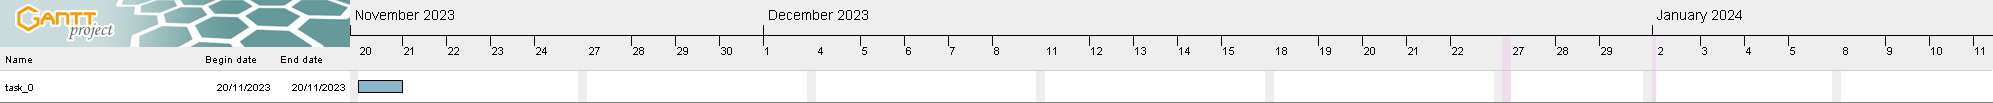
\includegraphics[width=1\textwidth]{gantt_chart.png}
        \label{fig:Gantt Chart}
    \end{figure}
\end{landscape}
\tikzstyle{every node}=[draw=black,thick,anchor=west]
\tikzstyle{selected}=[draw=red,fill=red!30]
\tikzstyle{optional}=[dashed,fill=gray!50]

\begin{document}

\begin{tikzpicture}[
                grow via three points={one child at (0.5,-0.7) and
                                two children at (0.5,-0.7) and (0.5,-1.4)},
                edge from parent path={(\tikzparentnode.south) |- (\tikzchildnode.west)}]

        \node {Computer Science Project}
        child { node {Project Initiation}
                        child { node {Define project scope and objectives}}
                        child { node {Identify stakeholders}}
                        child { node {Initial project meeting and setup}}
                }
        child [missing] {}
        child [missing] {}
        child [missing] {}
        child { node {Research and Analysis}
                        child { node {Conduct literature review}}
                        child { node {Define requirements}}
                        % Add more nodes as needed
                }
        % Continue with other project phases in similar fashion
        child { node {Design Phase}}
        child { node {Development Phase}}
        % ... and so on for other phases
        ;
\end{tikzpicture}
\section{Glossary}
\section{Marking Scheme}
\section{Changes to the Project Initiation Document}
\section{Current Environment Investigation Report}
\section{Requirements Specification}
\section{Design Report}
\section{Implementation}
\section{Testing}
\section{User Guide}
\section{Project Management}
\section{Meetings With Supervisor}
\section{Agile Development: Timebox 1}
\section{Agile Development: Timebox 2}
\section{Agile Development: Timebox 3}

\end{document}